\chapter{Information Retrieval}\label{Information_Retrieval}
Nel contesto dell'era moderna caratterizzata da un'enorme quantità di dati e informazioni disponibili, il campo dell'Information Retrieval (IR) emerge come un pilastro fondamentale per affrontare la sfida di estrarre conoscenza significativa da questa vastità di risorse. L'Information Retrieval si configura come un insieme di metodologie e processi volti a consentire agli individui di individuare, recuperare e accedere alle informazioni rilevanti all'interno di un mare di dati non strutturati.

Attraverso l'Information Retrieval, l'obiettivo primario è consentire agli utenti di navigare efficacemente attraverso l'abbondanza di informazioni, affiancando la loro esigenza di accesso immediato a contenuti rilevanti. L'Information Retrieval si pone come tramite tra gli individui e la vastità di dati disponibili, facilitando la traduzione delle esigenze degli utenti in query comprensibili e restituendo risultati pertinenti e significativi. In questo contesto, l'efficienza e l'accuratezza del processo di recupero dell'informazione diventano essenziali, influenzando direttamente l'esperienza dell'utente e la fruibilità delle risorse informative.

La continua crescita esponenziale delle risorse digitali, dai documenti di testo alle immagini, ai video e oltre, ha ampliato il campo dell'Information Retrieval, richiedendo soluzioni sempre più sofisticate ed efficienti per la ricerca e il recupero dei dati. Questa evoluzione ha portato alla coniugazione dell'Information Retrieval con discipline quali l'Intelligenza Artificiale, l'Apprendimento Automatico e l'Elaborazione del Linguaggio Naturale, che hanno apportato nuove prospettive e approcci innovativi al processo di recupero dell'informazione.

Nel seguito di questo capitolo, esploreremo le radici e l'evoluzione storica dell'Information Retrieval, analizzando come le sfide emergenti stiano plasmando il campo e delineando il panorama attuale in termini di approcci, tecnologie e prospettive future. Attraverso questa analisi, si prefigge l'obiettivo di evidenziare l'importanza cruciale dell'Information Retrieval nell'era moderna e la sua continua trasformazione nel contesto delle mutevoli esigenze informative degli individui.\section{Cos'è l'Information Retrieval} WIP
L'Information Retrieval rappresenta un campo interdisciplinare che si concentra sulla progettazione e lo sviluppo di metodologie, algoritmi e sistemi finalizzati a recuperare informazioni rilevanti da collezioni di dati eterogenei e spesso imponenti. A differenza dell'indicizzazione tradizionale dei dati, che organizza le risorse in base a criteri predefiniti, l'Information Retrieval mira a fornire agli utenti la capacità di formulare query personalizzate e ottenere risultati coerenti con le loro necessità informative.

Questo processo di recupero dell'informazione si basa su una serie di principi fondamentali. In primo luogo, gli utenti esprimono le loro richieste attraverso query, che possono essere composte da parole chiave, frasi o domande complete. L'Information Retrieval si impegna quindi a interpretare e comprendere le intenzioni sottostanti di queste query, cercando di identificare non solo le corrispondenze letterali, ma anche il contesto e il significato implicito. Successivamente, il sistema di Information Retrieval cerca all'interno della collezione di dati e documenti indicizzati per individuare quelli che meglio soddisfano le richieste dell'utente.

L'elemento chiave nell'Information Retrieval è la valutazione della rilevanza. Ogni documento recuperato viene valutato in base alla sua pertinenza rispetto alla query dell'utente. Tuttavia, la rilevanza è spesso un concetto sfumato e soggettivo, poiché può variare in base al contesto, all'utente e alle circostanze. Di conseguenza, molti sistemi di Information Retrieval utilizzano tecniche di ranking per ordinare i risultati in modo da presentare quelli più rilevanti o probabilmente interessanti all'utente in cima alla lista.

Un aspetto cruciale dell'Information Retrieval è la necessità di bilanciare l'efficienza e l'accuratezza. I sistemi di ricerca devono essere in grado di gestire grandi volumi di dati e rispondere rapidamente alle query degli utenti, garantendo al contempo che i risultati siano altamente pertinenti. Questa sfida ha portato allo sviluppo di algoritmi di ricerca e tecniche di indicizzazione sempre più sofisticati, che sfruttano modelli matematici, apprendimento automatico e processamento del linguaggio naturale per migliorare la qualità del recupero delle informazioni.

In sintesi, l'Information Retrieval svolge un ruolo cruciale nella navigazione dell'oceano di dati digitali, fornendo strumenti e metodologie per individuare e accedere alle informazioni desiderate. Questo campo continua a evolversi in risposta alla crescente complessità delle risorse informative e alle mutevoli aspettative degli utenti, spingendo verso l'adozione di approcci sempre più innovativi e tecnologicamente avanzati.
\section{La storia dell'Information Retrieval} WIP
L'evoluzione dell'Information Retrieval è intrecciata con lo sviluppo della tecnologia dell'informazione e delle comunicazioni. Dai primi sistemi basati su schede perforate e indici cartacei, si è passati gradualmente a sistemi digitali sempre più sofisticati. Uno dei punti di svolta storici è stato l'avvento dell'informatica, che ha reso possibile l'automatizzazione dei processi di recupero attraverso algoritmi e modelli matematici. Dagli anni '60 in poi, la crescita di Internet e il World Wide Web hanno ulteriormente trasformato il panorama dell'Information Retrieval, portando a sfide come l'eccesso di informazioni e la necessità di algoritmi di ranking sempre più avanzati. 
\section{I task dell'Information Retrieval} WIP
L'Information Retrieval comprende una serie di compiti interconnessi, ognuno dei quali mira a migliorare il processo di recupero delle informazioni. Tra questi task vi sono la classificazione dei documenti, l'indicizzazione (ovvero l'associazione di termini chiave ai documenti per facilitarne la ricerca), la rappresentazione dei documenti attraverso modelli matematici, il calcolo della similarità tra query e documenti, e l'ordinamento dei risultati in base alla loro rilevanza. Inoltre, l'Information Retrieval si è esteso alla ricerca multimediale, che coinvolge il recupero di dati come immagini e video.
\section{Lo stato dell'arte} WIP
Nel panorama contemporaneo, l'Information Retrieval (IR) è soggetto a un continuo processo di innovazione, spinto dalla rapida evoluzione delle tecnologie dell'informazione e dalle crescenti esigenze informative della società. L'IR sta affrontando sfide sempre più complesse, ma sta anche beneficiando di approcci e tecniche avanzate che stanno ridefinendo il modo in cui le informazioni vengono recuperate, elaborate e presentate agli utenti. Questa sezione esamina lo stato attuale dell'Information Retrieval, evidenziando le tendenze chiave e le tecnologie emergenti che stanno plasmando il campo.

\subsubsection{Approcci Basati su Apprendimento Automatico e Intelligenza Artificiale}
Un'evoluzione significativa nell'IR è l'ampio utilizzo dell'apprendimento automatico e dell'intelligenza artificiale per migliorare la precisione e la personalizzazione dei risultati di ricerca. Gli algoritmi di machine learning vengono addestrati su grandi insiemi di dati per comprendere le intenzioni degli utenti e valutare la rilevanza dei documenti. L'adozione di modelli neurali e reti neurali profonde (deep learning) ha portato a miglioramenti nella comprensione del linguaggio naturale e nella capacità di interpretare le query in modo più accurato.

\subsubsection{Ricerca Conversazionale e Interazione Uomo-Macchina}
L'IR sta sempre più abbracciando la ricerca conversazionale e l'interazione uomo-macchina. L'uso di assistenti vocali e chatbot basati su IR consente agli utenti di porre domande e ottenere risposte in modo più naturale e intuitivo. Questo richiede la comprensione di contesto, ambiguità e sfumature nelle query, oltre a fornire risposte coerenti e pertinenti.

\subsubsection{Ricerca Multimodale}
Con la crescente disponibilità di contenuti multimediali come immagini e video, l'IR si sta estendendo alla ricerca multimodale. Questo richiede l'elaborazione e l'integrazione di dati di diversi tipi, come testo, immagini e audio, per fornire risultati che riflettano la diversità dei contenuti presenti nelle collezioni digitali.

\subsubsection{Personalizzazione e Contestualizzazione}
L'IR sta diventando sempre più personalizzato, adattandosi alle preferenze e alle esigenze degli utenti individuali. I sistemi di raccomandazione basati su IR analizzano il comportamento passato dell'utente e forniscono risultati che sono più rilevanti e pertinenti per loro. Inoltre, la contestualizzazione sta guadagnando importanza, poiché i sistemi di IR cercano di comprendere il contesto in cui viene posta una query al fine di offrire risultati più precisi e utili.

\subsubsection{Etica, Privacy e Bias}
Con l'aumento dell'uso dell'IR, emergono preoccupazioni legate all'etica, alla privacy e ai bias. La personalizzazione e la profilazione degli utenti sollevano questioni sulla privacy e sulla gestione dei dati personali. Inoltre, l'IR deve affrontare il rischio di introdurre o amplificare bias culturali, politici o di genere nei risultati di ricerca, il che richiede un'attenzione crescente alla giustizia e all'equità nei sistemi di recupero dell'informazione.

In conclusione, lo stato dell'arte dell'Information Retrieval è caratterizzato da una fusione di approcci tradizionali e nuove tecnologie avanzate. L'adozione dell'apprendimento automatico, dell'intelligenza artificiale e la comprensione del contesto stanno ridefinendo l'esperienza di ricerca e recupero delle informazioni. Tuttavia, l'IR affronta anche sfide legate all'etica, alla privacy e all'equità, che richiedono attenzione continua. L'Information Retrieval rimane un campo dinamico e in evoluzione, destinato a plasmare ulteriormente il modo in cui le persone interagiscono con le informazioni nel mondo digitale in continua crescita.

\begin{center}
    \begin{figure}
        \centering
        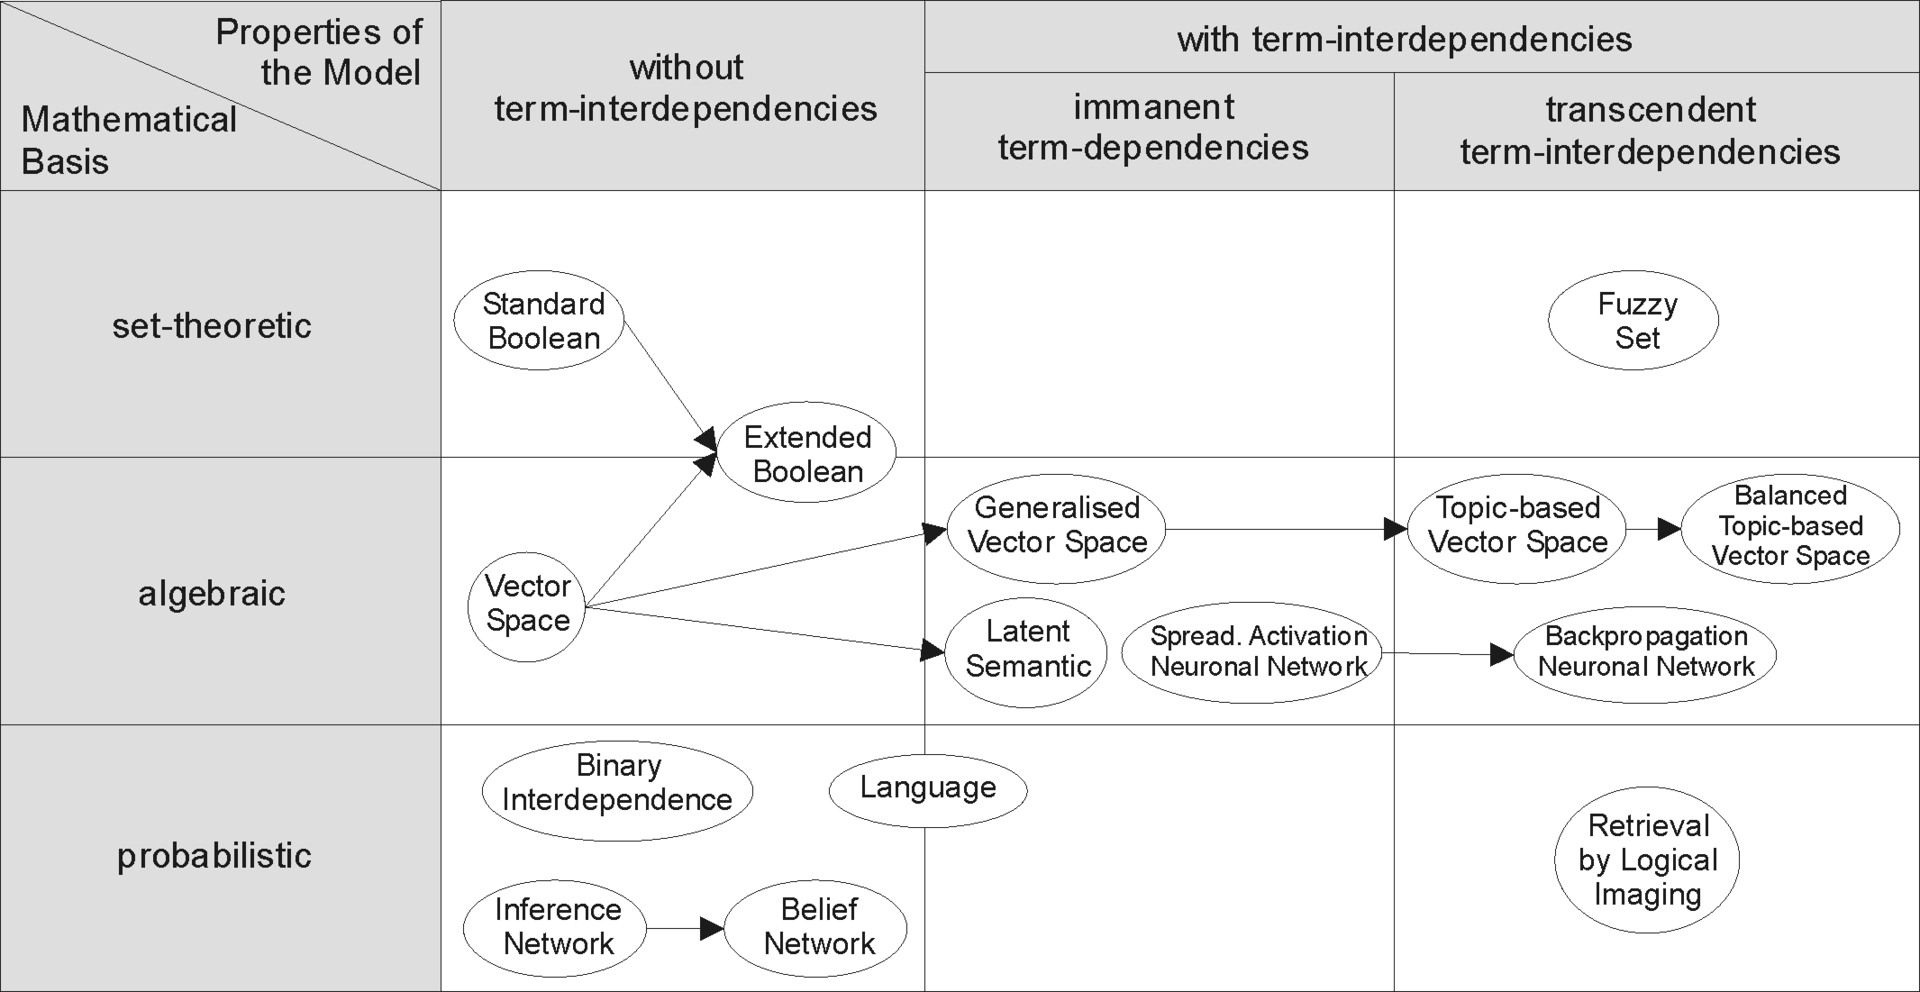
\includegraphics{images/typesofmodel.png}
        \caption{Tipi di modelli di Information Retrieval}
    \end{figure}
\end{center}